\documentclass{article}
\usepackage{amsmath,amssymb,graphicx,enumitem,wrapfig}

\begin{document}
\parindent=0cm
\parskip=6pt
\pagestyle{empty}

%Begin
%Language English
%Source Cariboo College High School Mathematics competition
%Title Final Round Part A 1974
%Question 1
%Subject arithmetic
%Category fractions
%Type MC
%Choices 5
%Answer C
%Creator Victor Semenoff
%Rdifficulty 25
%Qtext

\scriptsize
Source: Cariboo College High School Mathematics Contest

\normalsize
%\begin{wrapfigure}[2]{r}[0pt]{0pt}
%	\includegraphics[width=30mm,viewport=]{CCJ78-04}
%\end{wrapfigure}
The value of $\frac{(864)(866)-(864)(113)}{864-111}$ is:\\
%ChoiceA
(A) 111\\
%ChoiceB
(B) 113\\
%ChoiceC
(C) 864\\
%ChoiceD
(D) 866\\
%ChoiceE
(E) None of these.\\
%Ftext

%\begin{wrapfigure}{r}[0pt]{0pt}
%	\includegraphics[width=30mm,viewport=]{CCJ78-04}
%\end{wrapfigure}

\textbf{The correct answer is (C): 864}\\[1 ex]
\begin{align*}
\frac{(864)(866)-(864)(113)}{864-111}&=\frac{(864)(866-113)}{864-111}\\
=\frac{(864)(864+2-113)}{864-111}&=\frac{(864)(864-111)}{864-111}\\
&=864.
\end{align*}
%End
\\[5 ex]
%Begin
%Language English
%Source Cariboo College High School Mathematics competition
%Title Final Round Part A 1974
%Question 2
%Subject statistics
%Category concepts
%Type MC
%Choices 5
%Answer C
%Creator Victor Semenoff
%Rdifficulty 25
%Qtext

\scriptsize
Source: Cariboo College High School Mathematics Contest

\normalsize
%\begin{wrapfigure}[2]{r}[0pt]{0pt}
%	\includegraphics[width=30mm,viewport=]{CCJ78-04}
%\end{wrapfigure}
In a class there are 20 boys and 15 girls. On a certain test the average mark for the boys was 70, and the average mark for the girls was 84. The class average was:\\
%ChoiceA
(A) 74\\
%ChoiceB
(B) 75\\
%ChoiceC
(C) 76\\
%ChoiceD
(D) 77\\
%ChoiceE
(E) 78\\
%Ftext

%\begin{wrapfigure}{r}[0pt]{0pt}
%	\includegraphics[width=30mm,viewport=]{CCJ78-04}
%\end{wrapfigure}

\textbf{The correct answer is (C): 76}\\[1 ex]
Since there are 20 boys and the average mark received by the boys was 70, the sum of the marks received by the boys was $20\times70$. The sum of the marks received by the girls is $15\times84$. Thus the total sum of marks in the class is $20\times70+15\times84$, and because there are 35 total students the average grade is given by
\begin{equation*}
\frac{20\times70+15\times84}{35}=4\times10+3\times12=76.
\end{equation*}
%End
\\[5 ex]
%Begin
%Language English
%Source Cariboo College High School Mathematics competition
%Title Final Round Part A 1974
%Question 3
%Subject algebra
%Category concepts
%Type MC
%Choices 5
%Answer A
%Creator Victor Semenoff
%Rdifficulty 25
%Qtext

\scriptsize
Source: Cariboo College High School Mathematics Contest

\normalsize
%\begin{wrapfigure}[2]{r}[0pt]{0pt}
%	\includegraphics[width=30mm,viewport=]{CCJ78-04}
%\end{wrapfigure}
Define an operation$\star$ for numbers as $a\star b=\frac{a+2b}{2}.$ Then $(4\star2)\star3$ equals:\\
%ChoiceA
(A) 5\\
%ChoiceB
(B) $5\frac{1}{2}$\\
%ChoiceC
(C) 6\\
%ChoiceD
(D) $6\frac{1}{2}$\\
%ChoiceE
(E) None of these.\\
%Ftext

%\begin{wrapfigure}{r}[0pt]{0pt}
%	\includegraphics[width=30mm,viewport=]{CCJ78-04}
%\end{wrapfigure}

\textbf{The correct answer is (A): 5}\\[1 ex]
\begin{equation*}
(4\star2)\star3=(\frac{4+2\times2}{2})\star3=4\star3=\frac{4+2\times3}{2}=5.
\end{equation*}
%End
\\[5 ex]
%Begin
%Language English
%Source Cariboo College High School Mathematics competition
%Title Final Round Part A 1974
%Question 4
%Subject geometry
%Category area
%Type MC
%Choices 5
%Answer C
%Creator Victor Semenoff
%Rdifficulty 26
%Qtext

\scriptsize
Source: Cariboo College High School Mathematics Contest

\normalsize
\begin{wrapfigure}[5]{r}[0pt]{0pt}
	
\includegraphics[width=30mm,viewport=35 71 520 560]{CCFR74-4pic.eps}
\end{wrapfigure}
A side of the larger square shown is twice as long as a side of the smaller square, and the area of the shaded region is 20. If the inside square is made smaller by making each side $\frac{1}{2}$ as long, and the outside square is made larger by making each side twice as long, then the area of the shaded region will become:\\
%ChoiceA
(A) 50\\
%ChoiceB
(B) 80\\
%ChoiceC
(C) 105\\
%ChoiceD
(D) 160\\
%ChoiceE
(E) 165\\
%Ftext

\begin{wrapfigure}{r}[0pt]{0pt}
	
\includegraphics[width=30mm,viewport=35 71 520 560]{CCFR74-4pic.eps}
\end{wrapfigure}

\textbf{The correct answer is (C): 105}\\[1 ex]
Let $l$ be the length of the sides of the small square shown. The length of the sides of the large square will then be $2l$. The area of the shaded region is $(2l)^2-l^2=3l^2$, and thus we have $3l^2=20$ or $l^2=\frac{20}{3}$.

When the sides of the inside square are made $\frac{1}{2}$ as long, its area is $(\frac{1}{2}l)^2=\frac{1}{4}l^2$. When the sides of the outside square are made twice as long the area of the outside square will become $(4l)^2=16l^2$. The area of the new shaded region is now:
\begin{equation*}
16l^2-\frac{1}{4}l^2=\frac{63}{4}l^2=\frac{63}{4}\times \frac{20}{3}=105.
\end{equation*}
%End
\\[5 ex]
%Begin
%Language English
%Source Cariboo College High School Mathematics competition
%Title Final Round Part A 1974
%Question 5
%Subject algebra
%Category modelling
%Type MC
%Choices 5
%Answer D
%Creator Victor Semenoff
%Rdifficulty 26
%Qtext

\scriptsize
Source: Cariboo College High School Mathematics Contest

\normalsize
%\begin{wrapfigure}[2]{r}[0pt]{0pt}
%	\includegraphics[width=30mm,viewport=]{CCJ78-04}
%\end{wrapfigure}
Antonino travels 100 miles at $x$ miles per hour, 400 miles at $2x$ miles per hour, and 600 miles at $3x$ miles per hour. For the entire trip his average speed (in miles per hour) is:\\
%ChoiceA
(A) $\frac{1100x}{3}$\\
%ChoiceB
(B) $11x$\\
%ChoiceC
(C) $2x$\\
%ChoiceD
(D) $\frac{11x}{5}$\\
%ChoiceE
(E) $27x$\\
%Ftext

%\begin{wrapfigure}{r}[0pt]{0pt}
%	\includegraphics[width=30mm,viewport=]{CCJ78-04}
%\end{wrapfigure}

\textbf{The correct answer is (D): $\frac{11x}{5}$}\\[1 ex]
The time required for each part of the journey will equal the distance of that part divided by his speed during it. Thus the whole journey took
\begin{equation*}
\frac{100}{x}+\frac{400}{2x}+\frac{600}{3x}=\frac{500}{x}.
\end{equation*}
Since the total length was 1100 miles, the average speed is given by
\begin{equation*}
\frac{1100}{(\frac{500}{x})}=\frac{11x}{5}\textrm{mi}/\textrm{h}.
\end{equation*}
%End
\\[5 ex]
%Begin
%Language English
%Source Cariboo College High School Mathematics competition
%Title Final Round Part A 1974
%Question 6
%Subject arithmetic
%Category integers
%Type MC
%Choices 5
%Answer C
%Creator Victor Semenoff
%Rdifficulty 28
%Qtext

\scriptsize
Source: Cariboo College High School Mathematics Contest

\normalsize
%\begin{wrapfigure}[2]{r}[0pt]{0pt}
%	\includegraphics[width=30mm,viewport=]{CCJ78-04}
%\end{wrapfigure}
The number $54ab1$ is divisible by 9 and 11. The value of $2a+3b$ is:\\
%ChoiceA
(A) 19\\
%ChoiceB
(B) 20\\
%ChoiceC
(C) 21\\
%ChoiceD
(D) 22\\
%ChoiceE
(E) 23\\
%Ftext

%\begin{wrapfigure}{r}[0pt]{0pt}
%	\includegraphics[width=30mm,viewport=]{CCJ78-04}
%\end{wrapfigure}

\textbf{The correct answer is (C): 21}\\[1 ex]
For a number to be divisible by 9 the sum of the digits of that number must be divisible by 9. Thus $10+a+b$ must be divisible by 9, and since$0\leq a,b\leq9$,
\begin{equation*}
10+a+b=(18\textrm{or}27)
\end{equation*}
For a number to be divisible by 11 the sum of that number's digits with alternating sign must be divisible by 11. Thus $5-4+a-b+1=a-b+2$ must be divisible by 11, and therefore
\begin{equation*}
a-b+2=(11\textrm{or}0)
\end{equation*}
Adding the equations give
\begin{align*}
2a+12&=(18\textrm{or}27)+(11\textrm{or}0)=(29,18,38,\textrm{or}27)\\
a&=(\frac{17}{2},3,13,\textrm{or}\frac{15}{2})
\end{align*}
Since $a$ is a digit, we conclude $a=3$. Thus $b+13=(18\textrm{or}27)$, and since $0\leq b\leq9$ we have $b=5$. Therefore $2a+3b=6+15=21$.
%End
\\[5 ex]
%Begin
%Language English
%Source Cariboo College High School Mathematics competition
%Title Final Round Part A 1974
%Question 7
%Subject geometry
%Category area
%Type MC
%Choices 5
%Answer A
%Creator Victor Semenoff
%Rdifficulty 15
%Qtext

\scriptsize
Source: Cariboo College High School Mathematics Contest

\normalsize
\begin{wrapfigure}[4]{r}[0pt]{0pt}
	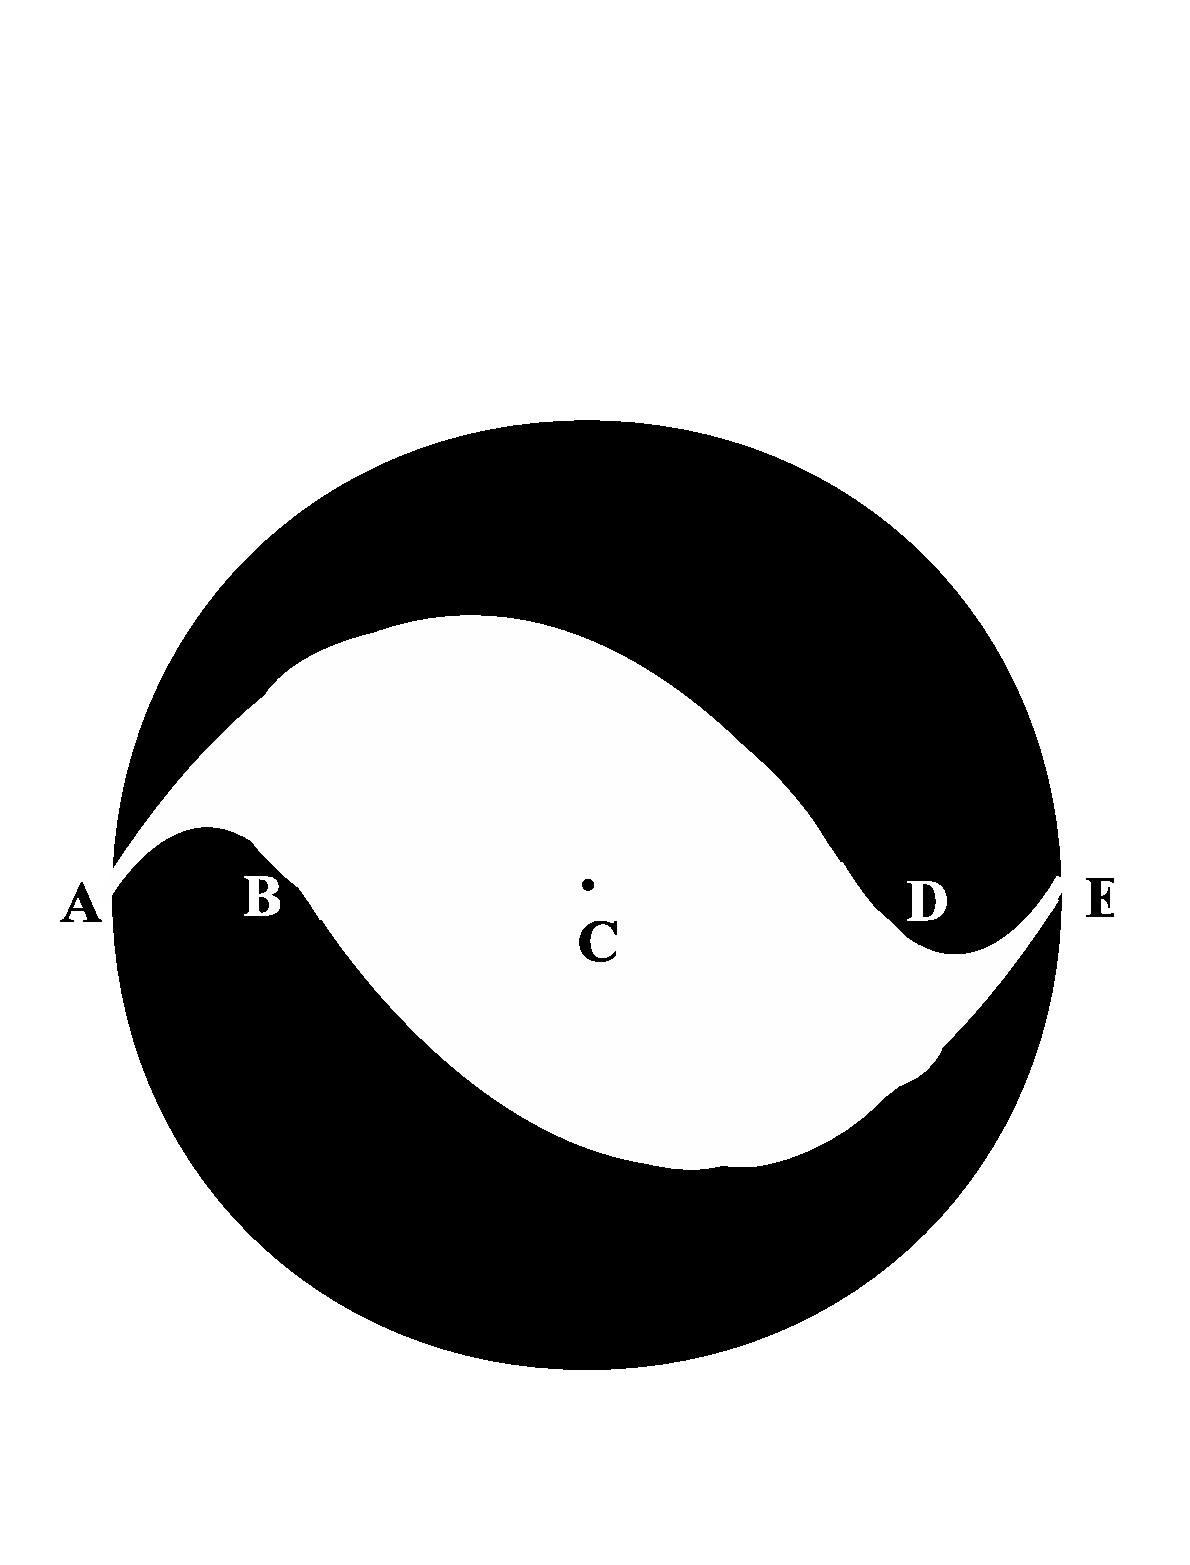
\includegraphics[width=30mm,viewport=16 80 533 545]{CCFR74-7pic.eps}
\end{wrapfigure}
The figure on the right may be obtained by drawing 6 semi-circles. If $AB=BC=CD=DE$, the area of the shaded section is $x$ and its perimeter is $y$, and the area and the circumference of the outside circle are $r$ and $s$, then $\frac{x}{r}+\frac{y}{s}$ equals:\\
%ChoiceA
(A) $\frac{1}{2}$\\
%ChoiceB
(B) 1\\
%ChoiceC
(C) 1$\frac{1}{2}$\\
%ChoiceD
(D) 2$\frac{1}{2}$\\
%ChoiceE
(E) $\frac{\pi}{2}$\\
%Ftext

\begin{wrapfigure}{r}[0pt]{0pt}
	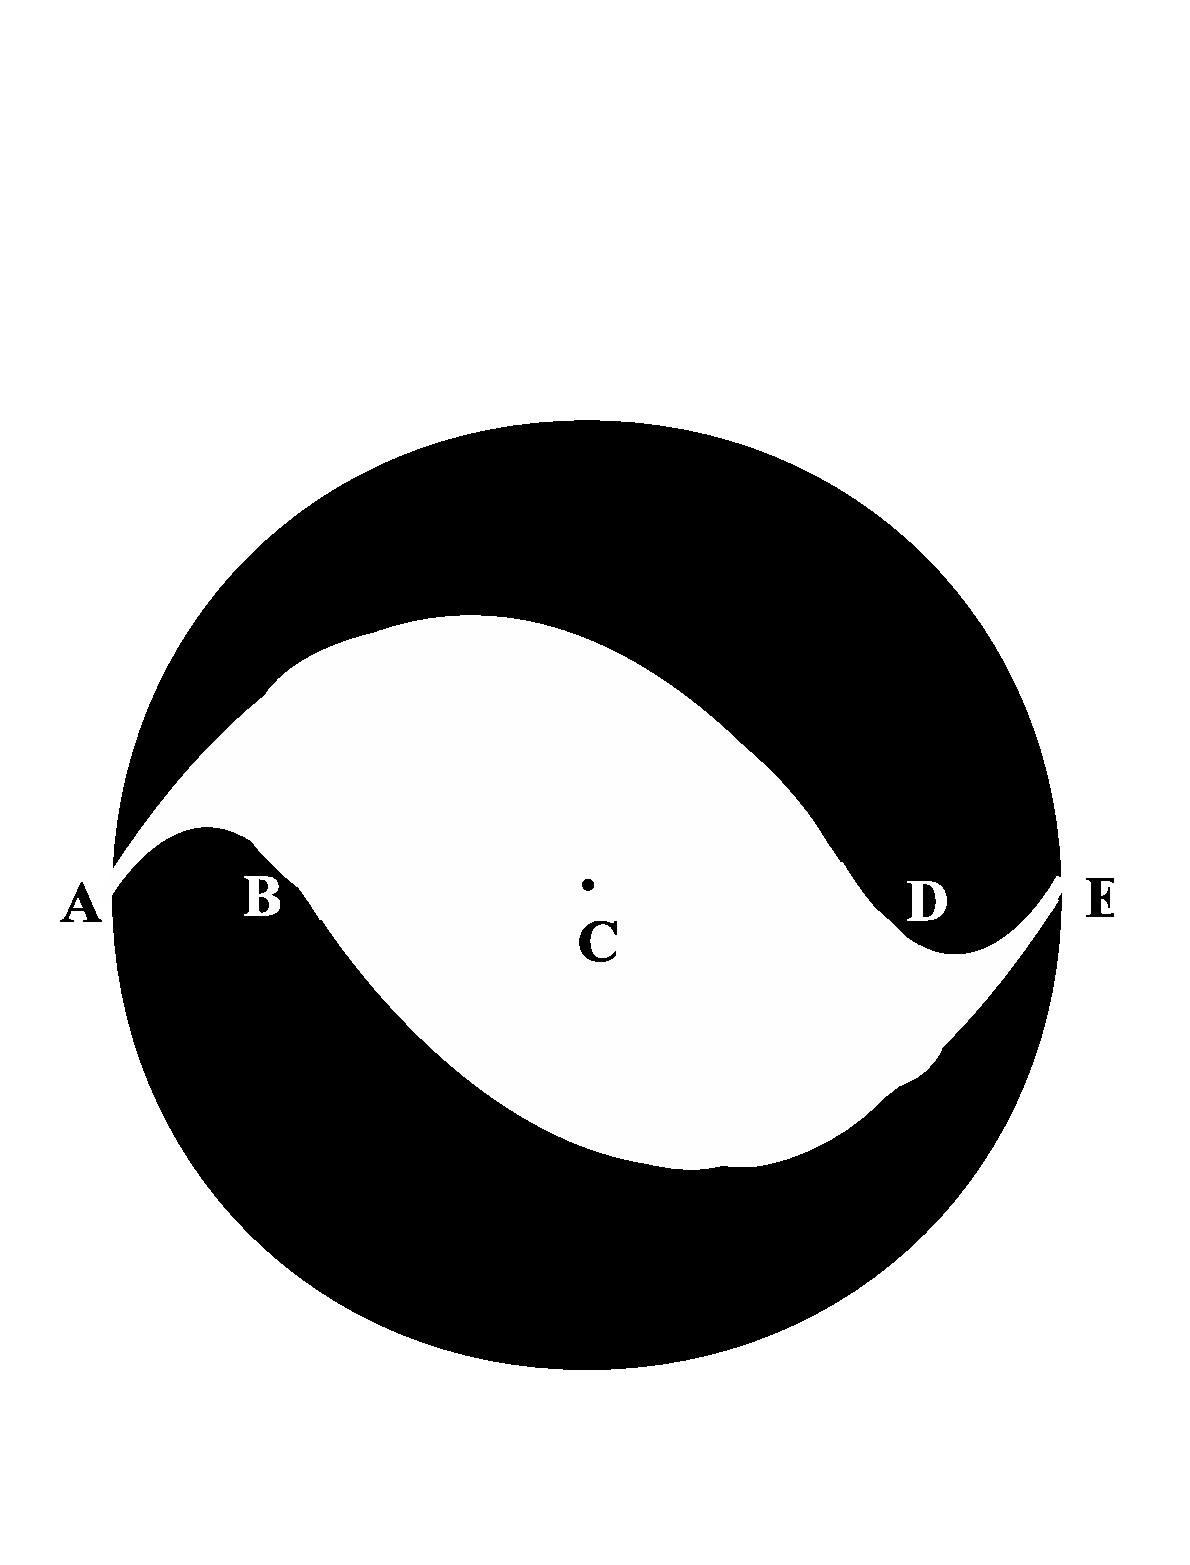
\includegraphics[width=30mm,viewport=16 80 533 545]{CCFR74-7pic.eps}
\end{wrapfigure}

\textbf{The correct answer is (C): $1\frac{1}{2}$}\\[1 ex]
The circumference of the large circle is $s=\pi 4AB$, while its area is $r=\pi(2AB)^2=4\pi(AB)^2$. The perimeter of the shaded region will be the sum of the lengths of the arcs $AD,AB,BE$, and $DE$. Thus
\begin{equation*}
y=\frac{1}{2}\pi3AB+\frac{1}{2}\pi AB+\frac{1}{2}\pi3AB+\frac{1}{2}\pi AB=4\pi AB.
\end{equation*}
The area of the shaded region will be twice the area of the semi-circle AD minus twice the area of the semi-circle AB (by symmetry). Thus
\begin{equation*}
x=2\times\frac{1}{2}\pi(\frac{3}{2}AB)^2-2\times\frac{1}{2}\pi(\frac{1}{2}AB)^2=2\pi(AB)^2.
\end{equation*}
Therefore
\begin{equation*}
\frac{x}{r}+\frac{y}{s}=\frac{2\pi(AB)^2}{4\pi(AB)^2}+\frac{4\pi AB}{4\pi AB}=\frac{1}{2}+1=1\frac{1}{2}.
\end{equation*}
%End
\\[5 ex]
%Begin
%Language English
%Source Cariboo College High School Mathematics competition
%Title Final Round Part A 1974
%Question 8
%Subject arithmetic
%Category integers
%Type MC
%Choices 5
%Answer E
%Creator Victor Semenoff
%Rdifficulty 27
%Qtext

\scriptsize
Source: Cariboo College High School Mathematics Contest

\normalsize
%\begin{wrapfigure}[2]{r}[0pt]{0pt}
%	\includegraphics[width=30mm,viewport=]{CCJ78-04}
%\end{wrapfigure}
It takes 1200 pieces of type to number the pages of a book. Each piece of type has one digit on it and is used only once. The number on the last page of the book is:\\
%ChoiceA
(A) 337\\
%ChoiceB
(B) 336\\
%ChoiceC
(C) 400\\
%ChoiceD
(D) 437\\
%ChoiceE
(E) 436\\
%Ftext

%\begin{wrapfigure}{r}[0pt]{0pt}
%	\includegraphics[width=30mm,viewport=]{CCJ78-04}
%\end{wrapfigure}

\textbf{The correct answer is (E): 436}\\[1 ex]
Each of the 9 pages from 1 to 9 will require 1 piece of type. Each of the $99-9=90$ pages from 10 to 99 will require 2 pieces of type. Each of the $n-99$ pages from 100 to $n$ will require 3 pieces of type. Thus the total required pieces of type will be
\begin{equation*}
1\times9+2\times90+3\times(n-99).
\end{equation*}
Since we are told 1200 pieces of type are required, we have
\begin{align*}
1\times9+2\times90+3\times(n-99)&=1200\\
3\times(n-99)&=1011\\
n&=436.
\end{align*}
%End
\\[5 ex]
%Begin
%Language English
%Source Cariboo College High School Mathematics competition
%Title Final Round Part A 1974
%Question 9
%Subject probability
%Category counting
%Type MC
%Choices 5
%Answer D
%Creator Victor Semenoff
%Rdifficulty 28
%Qtext

\scriptsize
Source: Cariboo College High School Mathematics Contest

\normalsize
%\begin{wrapfigure}[2]{r}[0pt]{0pt}
%	\includegraphics[width=30mm,viewport=]{CCJ78-04}
%\end{wrapfigure}
Marbles come in 10 different varieties, and there are 15 marbles in a pack. How many packs must a person buy to be sure of having at least 10 marbles of one variety?\\
%ChoiceA
(A) 17\\
%ChoiceB
(B) 11\\
%ChoiceC
(C) 10\\
%ChoiceD
(D) 7\\
%ChoiceE
(E) 2\\
%Ftext

%\begin{wrapfigure}{r}[0pt]{0pt}
%	\includegraphics[width=30mm,viewport=]{CCJ78-04}
%\end{wrapfigure}

\textbf{The correct answer is (D): 7}\\[1 ex]
If one purchased at most 6 packs of marbles, then one could conceivably end up with 9 marbles of each of the 10 varieties. On the other hand if one purchased 7 packs of marbles, one would have 105 marbles, which would be an average of 10.5 marbles in each of the 10 different varieties. Thus one must have at least 10 marbles in at least one variety
%End
\\[5 ex]
%Begin
%Language English
%Source Cariboo College High School Mathematics competition
%Title Final Round Part A 1974
%Question 10
%Subject algebra
%Category modelling
%Type MC
%Choices 5
%Answer B
%Creator Victor Semenoff
%Rdifficulty 30
%Qtext

\scriptsize
Source: Cariboo College High School Mathematics Contest

\normalsize
%\begin{wrapfigure}[2]{r}[0pt]{0pt}
%	\includegraphics[width=30mm,viewport=]{CCJ78-04}
%\end{wrapfigure}
How many multiples of 7 are there between one and one million that are even and also squares?\\
%ChoiceA
(A) 12\\
%ChoiceB
(B) 71\\
%ChoiceC
(C) 728\\
%ChoiceD
(D) 5,104\\
%ChoiceE
(E) 20,404\\
%Ftext

%\begin{wrapfigure}{r}[0pt]{0pt}
%	\includegraphics[width=30mm,viewport=]{CCJ78-04}
%\end{wrapfigure}

\textbf{The correct answer is (B): 71}\\[1 ex]
Each multiple of 7 that is even and also a square can be represented by $n^{2}7^{2}2^{2}$, where $n$ is a positive integer. Thus we must find $n$ such that
\begin{equation*}
n^{2}7^{2}2^{2}\leq1,000,000.
\end{equation*}
Solving for $n$ we get
\begin{align*}
n^2\leq \frac{10^6}{7^{2}2^{2}}&=\frac{2^{4}5^{6}}{7^2}\\
n\leq \frac{2^{2}5^{3}}{7}&=71\frac{3}{7}.
\end{align*}
Thus there will be 71 multiples of 7 between one and a million that are even and also squares.
%End
\\[5 ex]
%Begin
%Language English
%Source Cariboo College High School Mathematics competition
%Title Final Round Part B 1974
%Question 1
%Subject arithmetic
%Category integers
%Type SA
%Answer 17
%Creator Victor Semenoff
%Rdifficulty 28
%Qtext

\scriptsize
Source: Cariboo College High School Mathematics Contest

\normalsize
%\begin{wrapfigure}[2]{r}[0pt]{0pt}
%	\includegraphics[width=30mm,viewport=]{CCJ78-04}
%\end{wrapfigure}
The owner of the Go-Go bicycle shop was rather eccentric: when he took inventory, instead of counting the number of bicycles and tricycles in his shop, he counted the number of pedals and the number of wheels. If he counted 153 wheels and 136 pedals, how many tricycles did he have?\\
%Ftext

%\begin{wrapfigure}{r}[0pt]{0pt}
%	\includegraphics[width=30mm,viewport=]{CCJ78-04}
%\end{wrapfigure}

\textbf{The correct answer is 17}\\[1 ex]
Let $t$ be the number of tricycles he had, and $b$ be the number of bicycles. Since Each tricycle has 3 wheels and each bicycle has 2, we get
\begin{equation*}
3t+2b=153
\end{equation*}
Since both bicycles and tricycles have 2 pedals, we also have the equation
\begin{equation*}
2t+2b=136
\end{equation*}
Solving the two equations for $t$ we find $t=17$.
%End
\\[5 ex]
%Begin
%Language English
%Source Cariboo College High School Mathematics competition
%Title Final Round Part B 1974
%Question 2
%Subject arithmetic
%Category integers
%Type SA
%Answer 2521
%Creator Victor Semenoff
%Rdifficulty 27
%Qtext

\scriptsize
Source: Cariboo College High School Mathematics Contest

\normalsize
%\begin{wrapfigure}[2]{r}[0pt]{0pt}
%	\includegraphics[width=30mm,viewport=]{CCJ78-04}
%\end{wrapfigure}
What is the smallest whole number \textbf{larger than 1} which has a remainder of 1 when divided by 2,3,4,5,6,7,8,9, or 10?
%Ftext

%\begin{wrapfigure}{r}[0pt]{0pt}
%	\includegraphics[width=30mm,viewport=]{CCJ78-04}
%\end{wrapfigure}

\textbf{The correct answer is 2521}\\[1 ex]
For a number, $x$, to have a remainder of 1 when divided by $n$, $x$ must be one greater than a multiple of $n$. Thus the smallest number that will leave 1 as a remainder when divided by 2,3,4,5,6,7,8,9, or 10 will be 1 plus the lowest common multiple of these numbers. The prime factorizations of these are 2,3,$2^2$,5,$2\times3$,7,$2^3$,$3^3$, and $2\times5$ respectively. Thus the lowest common multiple is $2^3\times3^2\times5\times7=2520$, and the number we are looking for is 2521.
%End
\\[5 ex]
%Begin
%Language English
%Source Cariboo College High School Mathematics competition
%Title Final Round Part B 1974
%Question 3 Part A
%Subject algebra
%Category modelling
%Type SA
%Answer 120
%Creator Victor Semenoff
%Rdifficulty 27
%Qtext

\scriptsize
Source: Cariboo College High School Mathematics Contest

\normalsize
%\begin{wrapfigure}[2]{r}[0pt]{0pt}
%	\includegraphics[width=30mm,viewport=]{CCJ78-04}
%\end{wrapfigure}
A rancher is due to deliver a truckload of cattle to Kamloops. He decides he should arrive at exactly 11:00 am. If the truck averaged 30 mi/h, it would arrive at ten, an hour early; at 20 mi/h it would arrive at noon, an hour late. How far (in miles) is the ranch from the city? 
%Ftext

%\begin{wrapfigure}{r}[0pt]{0pt}
%	\includegraphics[width=30mm,viewport=]{CCJ78-04}
%\end{wrapfigure}

\textbf{The correct answer is 120}\\[1 ex]
Let $d$ be the distance, $v_f=30$ mi/h and $v_s=20$ mi/h. The difference in the times for each trip is given by
\begin{equation*}
\frac{d}{v_s}-\frac{d}{v_f}=2\textrm{hr}.
\end{equation*}
Solving for $d$ we find
\begin{align*}
d(v_f-v_s)&=2\times v_f \times v_s\\
d(10)&=2\times20\times30\\
d&=120\textrm{mi}.
\end{align*}
%End
\\[5 ex]
%Begin
%Language English
%Source Cariboo College High School Mathematics competition
%Title Final Round Part B 1974
%Question 3 Part B
%Subject algebra
%Category modelling
%Type SA
%Answer 24
%Creator Victor Semenoff
%Rdifficulty 28
%Qtext

\scriptsize
Adapted From: Cariboo College High School Mathematics Contest

\normalsize
%\begin{wrapfigure}[2]{r}[0pt]{0pt}
%	\includegraphics[width=30mm,viewport=]{CCJ78-04}
%\end{wrapfigure}
A rancher is due to deliver a truckload of cattle to Kamloops   . He decides he should arrive at exactly 11:00 am. If the truck averaged 30 mi/h, it would arrive at ten, an hour early; at 20 mi/h it would arrive at noon, an hour late. At what speed (in mi/h) would he need to drive to arrive on time? 
%Ftext

%\begin{wrapfigure}{r}[0pt]{0pt}
%	\includegraphics[width=30mm,viewport=]{CCJ78-04}
%\end{wrapfigure}

\textbf{The correct answer is 24}\\[1 ex]
Let $t$ be the time for the trip if he arrived on time. $d$ be the distance, $v_f=30$ mi/h and $v_s=20$ mi/h. The difference in the times for each trip is given by
\begin{equation*}
\frac{d}{v_s}-\frac{d}{v_f}=2\textrm{hr}.
\end{equation*}
Solving for $d$ we find
\begin{align*}
d(v_f-v_s)&=2\times v_f \times v_s\\
d(10)&=2\times20\times30\\
d&=120\textrm{mi}.
\end{align*}
The time for the longer trip is then given by $\frac{d}{v_s}=t+1$, thus $t=\frac{120}{20}-1=5$ hr. Therefore, he would have to drive $\frac{120}{5}=24$ mi/hr to arrive on time.
%End
\end{document}
